\chapter{Procesos láser}

\section{Conceptos básicos de tecnología láser}

\subsection{Introducción}

Fundamentalmente, un láser es luz, es decir, un flujo de partículas denominadas \textbf{fotones}. La forma más común con la que nos relacionamos con esta radiación electromagnética es la \textbf{luz difusa}, que nos permite percibir el mundo que nos rodea.

Esta luz difusa se compone de múltiples ondas electromagnéticas, cada una con su propia frecuencia, amplitud y fase, resultantes de la interacción de fotones generados por alguna fuente, como el Sol, con la materia. La luz visible, es decir, la que nuestros ojos pueden detectar, se encuentra aproximadamente entre los 380 y 750 nanómetros de longitud de onda, formando el espectro de colores observable.

En contraste con la luz difusa, un láser presenta tres propiedades fundamentales: es \textbf{monocromático}, compuesto por ondas de una única frecuencia; \textbf{coherente}, con ondas en fase entre sí; y \textbf{direccional}, ya que se propaga predominantemente en un solo sentido y dirección (Figura \ref{laigfig}). 

El término \textbf{LASER} es un acrónimo del inglés \textit{Light Amplification by Stimulated Emission of Radiation}, que en español significa \textit{amplificación de luz por emisión estimulada de radiación}. Como indica el acrónimo, el principio clave detrás de un láser es la \textbf{emisión estimulada}, fenómeno predicho por Albert Einstein en 1917.

De manera simplificada, la emisión estimulada ocurre cuando un fotón incide sobre un átomo o molécula que se encuentra en un estado energético excitado. Este impacto provoca que la partícula decaiga a un nivel energético inferior, emitiendo un fotón con \textbf{las mismas características} (frecuencia, fase y dirección) que el fotón incidente. La superposición de estos fotones idénticos genera \textbf{interferencia constructiva}, resultando en la amplificación de la luz, base del funcionamiento de cualquier láser (Figura \ref{emisfig}).

\begin{figure}[h!]
	\centering
	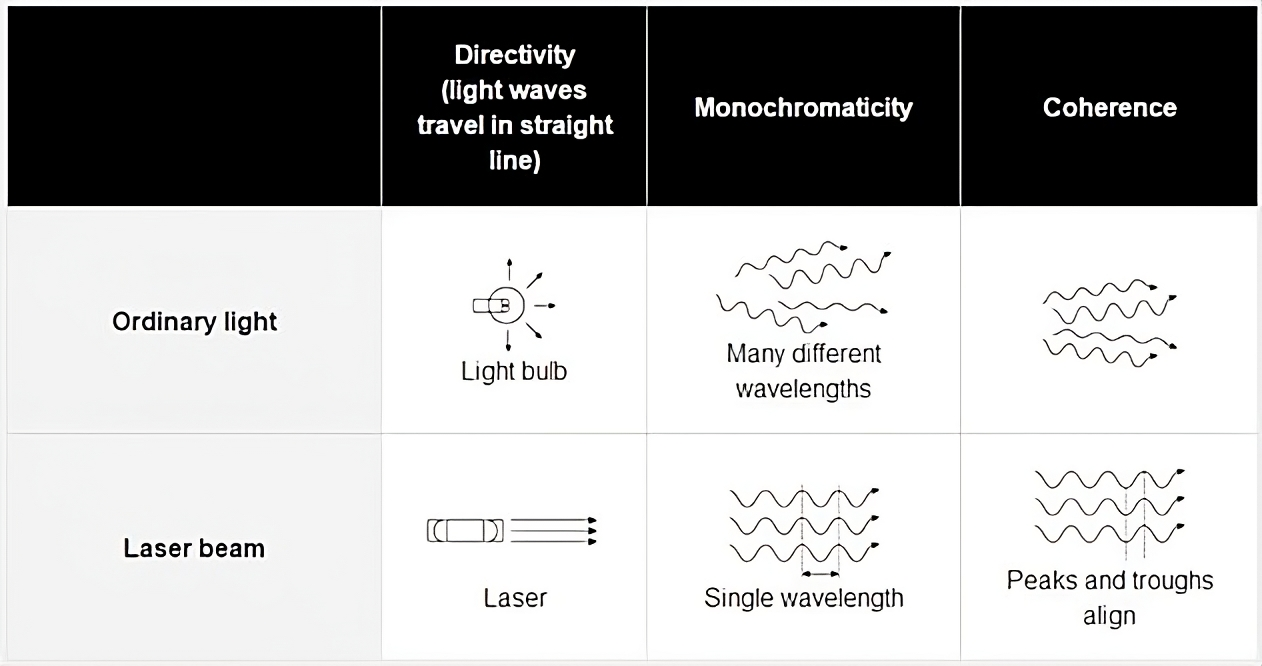
\includegraphics[width=0.7\linewidth]{imgs/laig.png}
	\caption{Luz difusa comparada con luz láser. \href{https://triumphlaser.com/differences-ordinary-light-laser-beams/}{Fuente}}
	\label{laigfig}
\end{figure}

Si bien el principio de emisión estimulada fue predicho por Albert Einstein en 1917, en el contexto de sus estudios sobre la radiación del cuerpo negro y la formulación de la ley de Planck, no fue hasta 1960 cuando Theodore H. Maiman construyó el primer láser propiamente tal. Este dispositivo utilizaba un cristal de rubí (\textit{Al$_2$O$_3$:Cr$^{3+}$}) como medio activo, excitado mediante una lámpara de destello, y emitía un haz de luz roja con una longitud de onda de aproximadamente 694 nm.

\begin{figure}[h!]
	\centering
	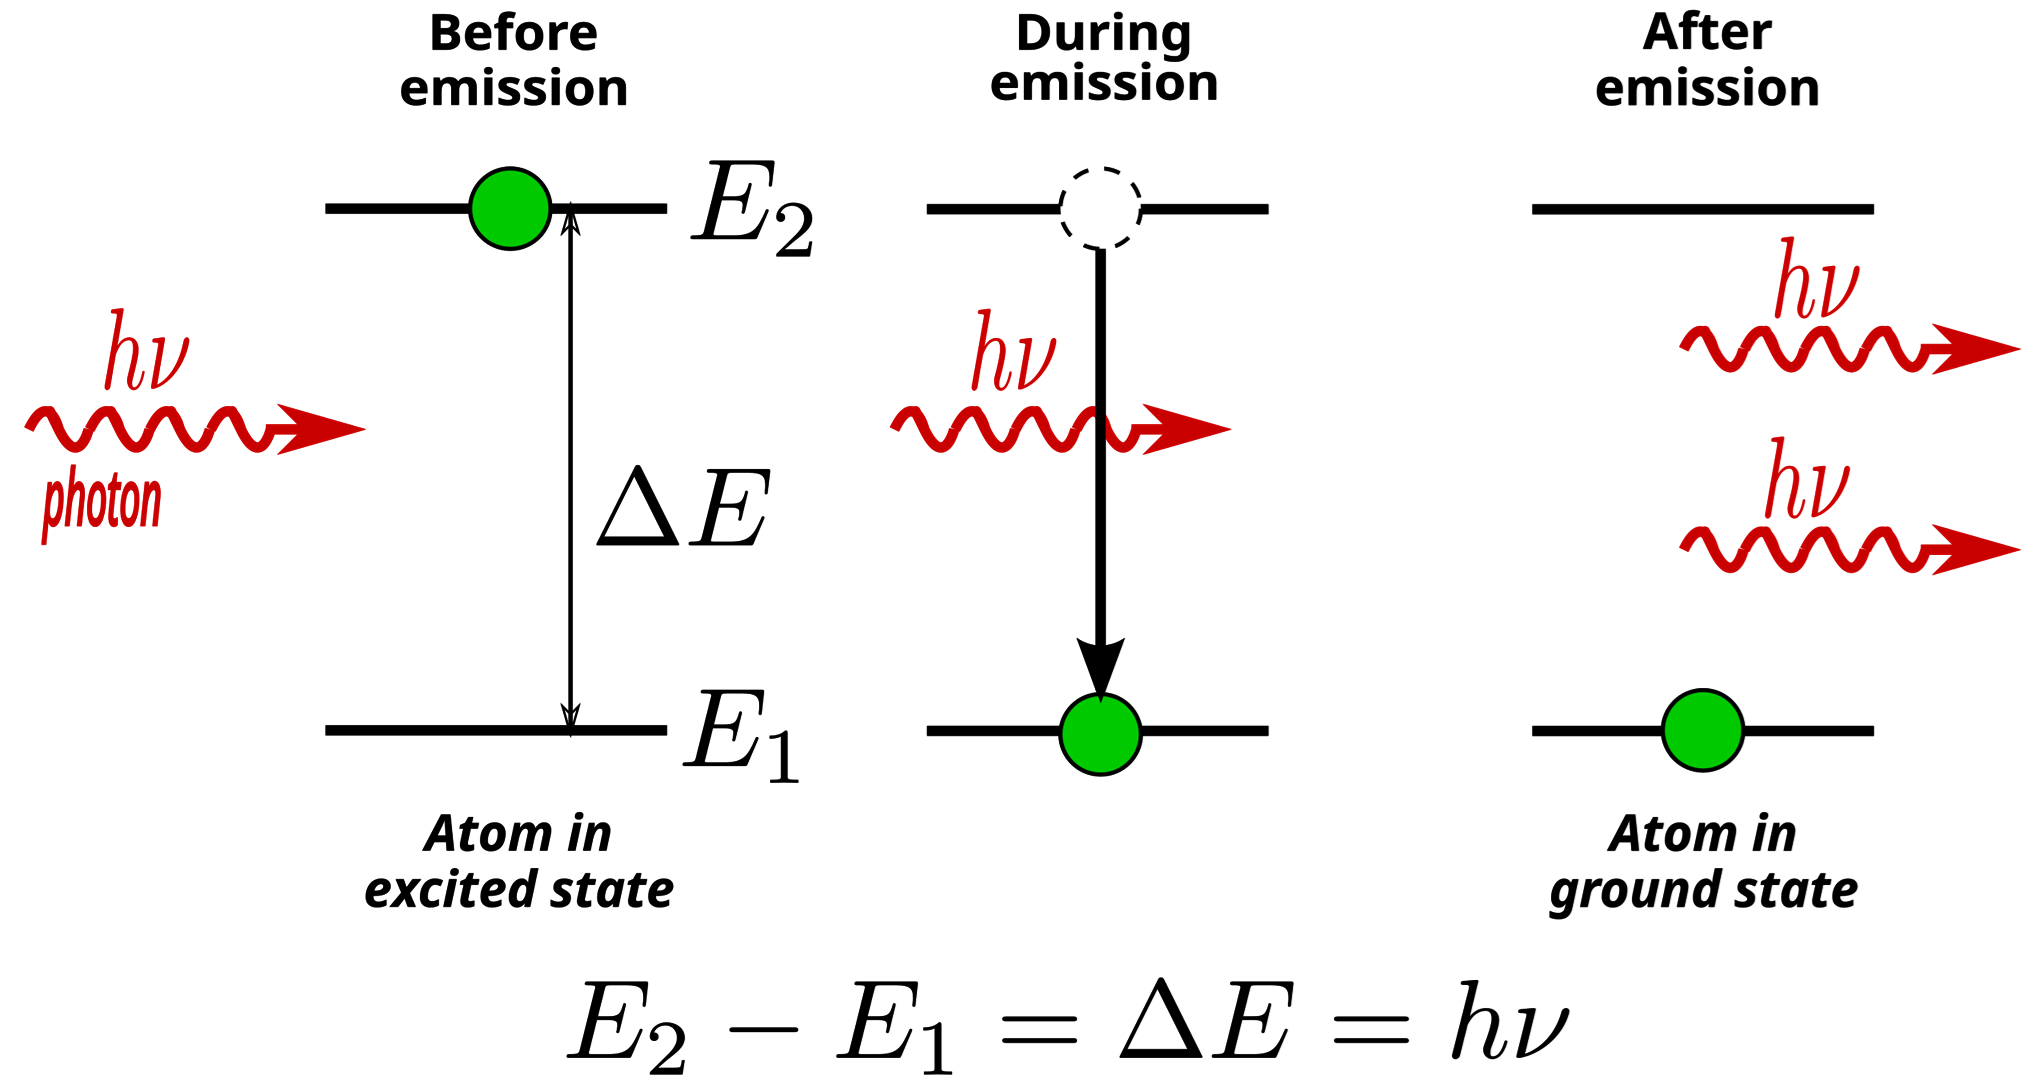
\includegraphics[width=0.7\linewidth]{imgs/emstimu.png}
	\caption{Emisión estimulada de luz. \href{https://en.wikipedia.org/wiki/Stimulated_emission}{Fuente}}
	\label{emisfig}
\end{figure}

Al momento de su desarrollo, el láser no respondía a una necesidad tecnológica específica, por lo que fue descrito por algunos como \comillas{una solución en busca de un problema}. Sin embargo, su potencial pronto se reconoció en múltiples campos, desde las comunicaciones ópticas hasta la manufactura de alta precisión.

El haz láser puede generarse y amplificarse hasta alcanzar altas densidades de energía; sin embargo, la generación constituye solo una parte del proceso. Para que esta energía se utilice de manera efectiva, es necesario guiar, enfocar y controlar la propagación de la luz, tareas propias de la \textbf{óptica}. Mediante sistemas de espejos, lentes, prismas o fibras ópticas, el haz puede dirigirse con gran precisión y concentrarse en áreas extremadamente pequeñas.

De esta manera, un láser puede considerarse como una herramienta capaz de concentrar una alta densidad de energía en un punto extremadamente reducido, el cual llamaremos \textbf{spot láser}, y así, modificar materiales —ya sea mediante corte, grabado o tratamientos superficiales— a través de mecanismos predominantemente térmicos.

El principio de este proceso presenta ventajas significativas, ya que posibilita trabajar una amplia variedad de materiales sin depender de su resistencia o dureza mecánica, y sin aplicar fuerzas de contacto, a diferencia de los procesos de mecanizado convencionales, como el corte por CNC. No obstante, la naturaleza térmica de la interacción puede generar efectos no deseados en el material, tales como la alteración de la microestructura, la formación de zonas afectadas por el calor o la aparición de defectos que comprometen la calidad final de la pieza.

\subsection{Partes de un de corte sistema láser}

Una máquina de corte láser combina los subsistemas típicos de una máquina de control numérico (CNC) con los componentes específicos necesarios para el funcionamiento de la herramienta láser (Figura \ref{lasisfig}). 

\begin{figure}[h!]
	\centering
	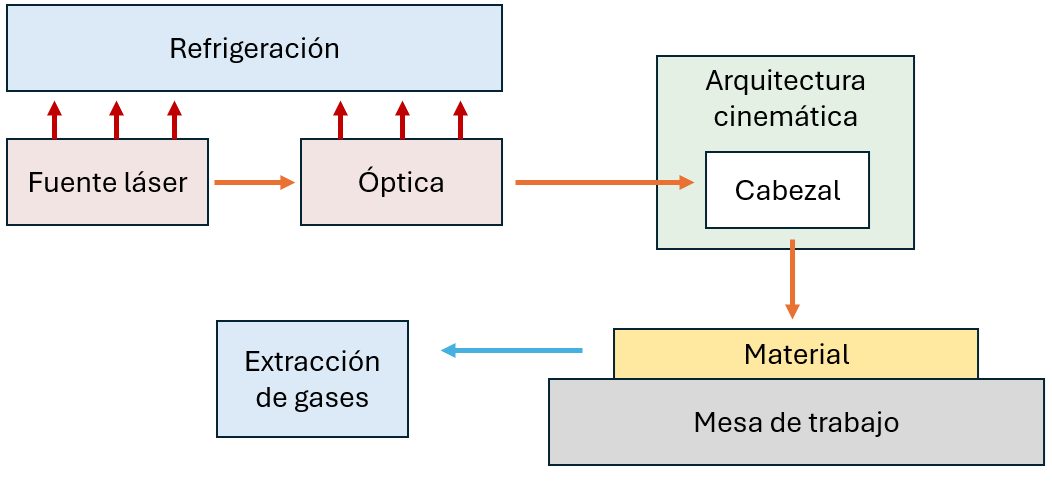
\includegraphics[width=0.8\linewidth]{imgs/lasis.png}
	\caption{Diagrama general de un sistema láser.}
	\label{lasisfig}
\end{figure}


Entre los principales se incluyen:

\begin{itemize}
	\item \textbf{Fuente láser}: conjunto de componentes encargados de transformar la energía eléctrica en radiación láser mediante los procesos de \textbf{emisión estimulada}. Existen diferentes tipos de fuentes, cada una con características particulares de potencia, longitud de onda y eficiencia.
	
	\item \textbf{Sistema de transmisión óptica}: conjunto de elementos que permiten guiar y enfocar el haz de fotones desde la fuente hasta la superficie de trabajo. Dependiendo del tipo de láser, esta transmisión puede realizarse mediante \textbf{espejos, lentes y/o fibras ópticas}.
\end{itemize}

La integración de estos subsistemas hace necesaria la inclusión de otros subsistemas auxiliares importantes:  

\begin{itemize}
	\item \textbf{Sistema de refrigeración:} Disipa las altas cantidades de calor generadas tanto en la fuente como en los elementos ópticos. En equipos industriales modernos, los láseres más avanzados pueden alcanzar potencias de salida superiores a \textbf{120 kW}, con eficiencias eléctricas entre \textbf{30\% y 45\%}, según la tecnología empleada. Esto refleja la gran densidad energética involucrada y la necesidad de un control térmico riguroso para mantener la estabilidad y calidad del haz.  
	
	\item \textbf{Sistema de ventilación y extracción de gases:} el trabajo con láser puede generar vapores y gases tóxicos o corrosivos que afectan tanto la salud humana como la maquinaria. Particularmente crítica es la protección de los elementos ópticos cercanos a la zona de trabajo, que pueden dañarse por la acumulación de partículas o condensados.
\end{itemize}

Además, las máquinas incluyen los subsistemas comunes de cualquier equipo de fabricación digital, tales como controlador, servomotores, transmisión, chasis y dispositivos de seguridad.  

Por lo general, las máquinas de corte láser operan sobre un sistema cartesiano de movimiento en el plano XY, mediante el cual se desplaza el cabezal óptico sobre la pieza de trabajo. Esta configuración permite realizar cortes bidimensionales y es la más común en aplicaciones industriales de corte y grabado.  

Mantener la distancia focal óptima es esencial para asegurar un proceso estable y controlado. Por ello, muchos equipos incorporan ajustes en el eje Z, ya sea mediante el movimiento de la bandeja de trabajo, el desplazamiento del cabezal o modificaciones en el sistema óptico de enfoque. Esta distancia puede regularse en tiempo real mediante distintos tipos de sensores: capacitivos, para materiales metálicos, u ópticos e infrarrojos, para materiales no metálicos.  

Finalmente, las propiedades del material determinan qué \textbf{tecnología láser} resulta más adecuada. En la práctica industrial, estas se clasifican de manera coloquial como \textbf{láser de $\mathrm{CO_2}$}, utilizado principalmente para materiales no metálicos, o \textbf{láser de fibra}, orientado a metales, aunque estas denominaciones simplifican conceptos más complejos sobre la generación y transmisión del haz láser.

\subsection{Generación del láser}

La \textbf{fuente láser} es el subsistema encargado de generar y amplificar el haz de luz coherente que caracteriza a cualquier sistema láser. Esta fuente se compone principalmente de tres elementos fundamentales: el \textbf{medio activo}, el \textbf{mecanismo de bombeo} o excitador, y el \textbf{resonador óptico}.

\begin{figure}[h!]
	\centering
	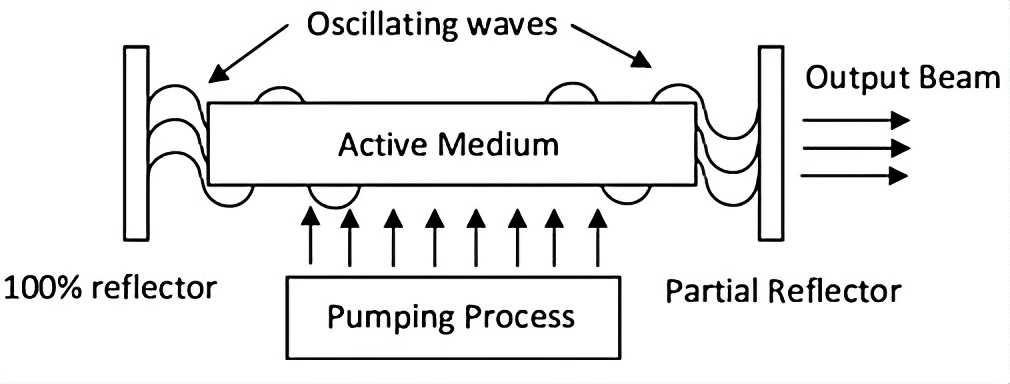
\includegraphics[width=0.7\linewidth]{imgs/laspart.png}
	\caption{Partes de una fuente láser. \href{https://www.researchgate.net/publication/281235580_Laser_Physics}{Fuente}}
	\label{laspartfig}
\end{figure}


El \textbf{medio activo} es el material en el cual se produce la emisión estimulada, y determina las características fundamentales del láser, en particular su frecuencia o longitud de onda. Esta propiedad es esencial al seleccionar la tecnología láser adecuada para un proceso específico, pues la interacción con el material objetivo depende de la frecuencia.

El medio activo puede encontrarse en distintos estados de la materia (sólido, líquido o gaseoso), cada uno con ventajas particulares según la aplicación. En el Cuadro \ref{tab:medios} se presenta un resumen de los medios activos más comúnmente utilizados en la industria.

\begin{table}[h!]
	\centering
	\small
	\caption{Medios activos más utilizados en láseres industriales}
	\label{tab:medios}
	\begin{tabular}{|l|p{3cm}|p{3cm}|p{3cm}|p{3cm}|}
		\hline
		& \textbf{Diodo láser} & \textbf{Nd:YAG} & \textbf{Fibra Yb} & \textbf{CO$_2$} \\ \hline
		Estado & Sólido / Semiconductor & Sólido & Sólido / Fibra & Gas \\ \hline
		$\lambda$ ($\mu$m) & 0.4–2.0 & 1.064 & 1.03–1.08 & 10.6 \\ \hline
		Bombeo & Eléctrico & Óptico / Eléctrico & Eléctrico / Diodo & Eléctrico (descarga) \\ \hline
		Aplicaciones & Grabado, comunicaciones ópticas, bombeo de otros láseres & Corte y soldadura de metales, grabado industrial & Corte y soldadura de metales, alta eficiencia & Corte y grabado de materiales no metálicos \\ \hline
	\end{tabular}
\end{table}


Para que el medio activo emita fotones mediante \textbf{emisión estimulada}, primero es necesario elevar los electrones de sus átomos o iones a estados energéticos superiores. Según la teoría cuántica de Planck, estos niveles de energía son discretos. En la práctica, en materiales reales los niveles no son estrictamente discretos, sino que se presentan como \textbf{bandas energéticas} que facilitan la interacción entre partículas.

El proceso que suministra la energía necesaria para excitar a los electrones se denomina \textbf{mecanismo de bombeo} o excitador. Este puede ser de naturaleza óptica o eléctrica, según la fuente utilizada:

\begin{itemize}
	\item \textbf{Excitación óptica:} consiste en la inyección de luz externa, generalmente proveniente de lámparas de destello o diodos láser.
	\item \textbf{Excitación eléctrica:} se logra mediante descargas eléctricas que transfieren energía directamente al medio activo, común en láseres de gas o de semiconductor.
\end{itemize}

El bombeo debe ser suficiente para alcanzar un fenómeno crítico denominado \textbf{inversión de población}, en el cual el número de partículas en estado excitado supera al de las partículas en estado fundamental (Figura \ref{invpopfig}). La inversión de población es la condición indispensable para que la emisión estimulada predomine sobre la emisión espontánea y permita la amplificación coherente de la luz.


\begin{figure}[h!]
	\centering
	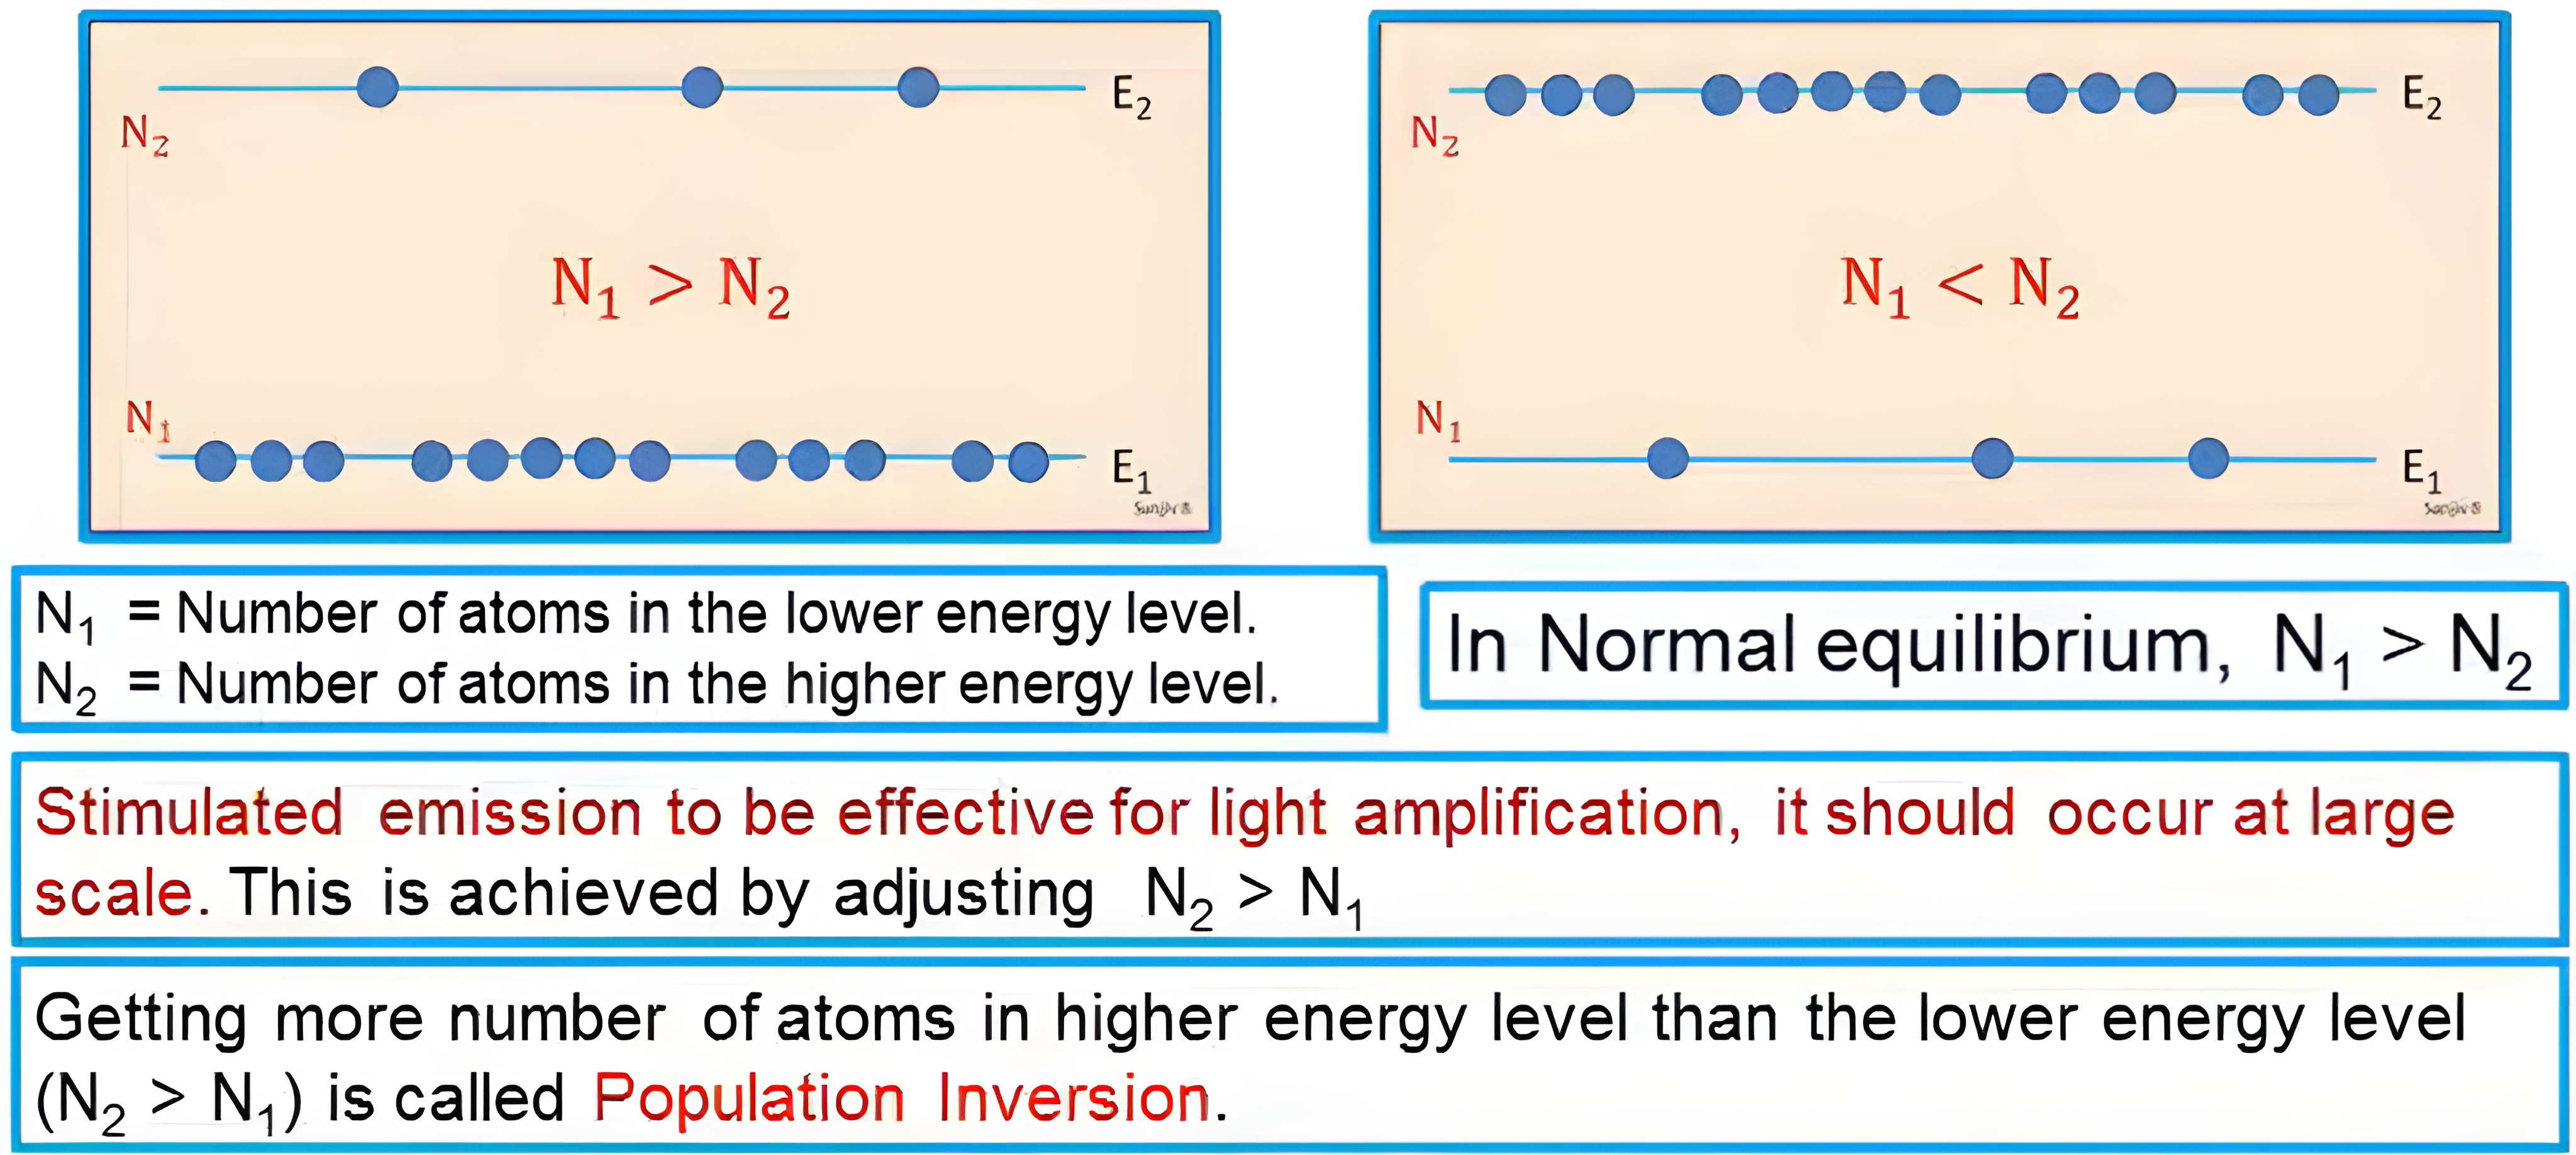
\includegraphics[width=0.8\linewidth]{imgs/invpop.png}
	\caption{Inversión de población hacia estado estimulado. \href{https://www.youtube.com/watch?v=Gw0fvPeVh9s}{Fuente}}
	\label{invpopfig}
\end{figure}

Al inicio del proceso láser, una pequeña fracción de electrones decae espontáneamente, generando los primeros fotones. Estos fotones actúan como \textbf{semillas}, estimulando a otros electrones excitados y dando lugar a un efecto en cadena que produce el haz coherente característico del láser. 

No todos los electrones excitados experimentan emisión estimulada. Algunos decaen de manera espontánea hacia otros estados, incluidos estados metaestables, o liberan su energía sin generar fotones, por ejemplo, mediante la creación de fonones, que se manifiestan como calor. Estos procesos representan una fuente de pérdidas e ineficiencia en el sistema láser, ya que el aumento de temperatura reduce la proporción de decaimientos estimulados efectivos. Por esta razón, la refrigeración adecuada del medio activo es fundamental para mantener la eficiencia y la estabilidad del haz láser durante su operación.

Dado que la probabilidad de interacción entre los fotones y los electrones es relativamente baja, se incorpora el \textbf{resonador óptico}. Este componente, conformado típicamente por espejos, refleja repetidamente el haz dentro del medio activo, incrementando la probabilidad de emisiones estimuladas y, por ende, la densidad de fotones coherentes. Uno de los espejos del resonador es parcialmente reflectante, permitiendo que parte del haz generado escape y constituya el láser útil, que posteriormente se dirige a través del sistema óptico hacia la aplicación deseada.

\section{Óptica}

\subsection{Interacción con la materia}

Al incidir sobre un material, una onda electromagnética puede experimentar tres fenómenos principales, que dependen tanto de las propiedades de la luz como de las características del material: \textbf{absorción} (\(A\)), \textbf{reflexión} (\(R\)) y \textbf{transmisión o refracción} (\(T\)) (Figura \ref{reflepfig}). Normalizando la energía del rayo incidente como el total, se cumple:

\begin{equation}
	A + R + T = 1
\end{equation}

La distribución de estos valores dependerá en gran parte de la frecuencia de la onda y de las propiedades del material. Así, si un material no transmite la radiación incidente, se dirá que es \textbf{opaco} a esa longitud. Mientras que si transmite la mayor parte, se llamará \textbf{transparente} a esa longitud.

\begin{figure}[h!]
	\centering
	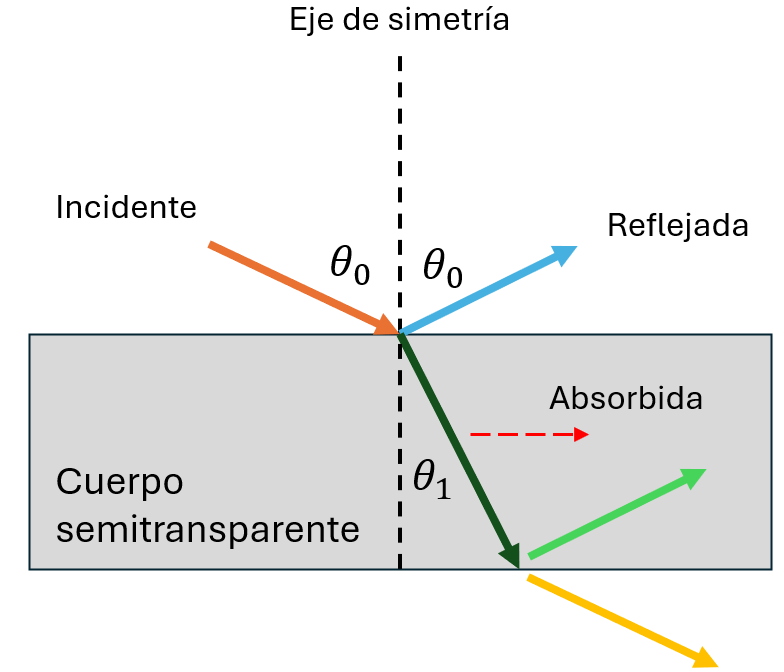
\includegraphics[width=0.5\linewidth]{imgs/reflep.png}
	\caption{Diagrama de interacción de la radiación con materia semitransparente.}
	\label{reflepfig}
\end{figure}

En el caso de materiales opacos, como la transmisión es despreciable (\(T \approx 0\)), la energía se distribuye únicamente entre absorción y reflexión. Por lo tanto, el coeficiente de absorción \(A\) de un material se suele determinar de manera indirecta, midiendo la energía reflejada.  

En la Figura \ref{absfig} se muestran los coeficientes de absorción de distintos materiales en función de la longitud de onda de varias fuentes láser. Se observa claramente la preferencia del láser de \(\mathrm{CO_2}\) para materiales inorgánicos, mientras que el láser de fibra Yb es más eficiente con metales. 

Como se muestra en la Figura \ref{hotafig}, el coeficiente de absorción puede aumentar radicalmente con el cambio de fase de un material. Esto se explica por el reordenamiento en la estructura molecular, y por tanto, de la configuración electrónica, creando nuevos niveles de energía y permitiendo absorber fotones que antes eran incompatibles.

Desde el punto de vista de la eficiencia, la absorción constituye un parámetro crítico en la selección de un sistema láser, ya que se busca maximizarla en la pieza de trabajo. Por el contrario, los mecanismos de transmisión óptica están diseñados para minimizar la absorción en los componentes, buscando maximizar la reflexión (en espejos) o la transmisión y luego reflexión (en lentes y fibras ópticas).  

\begin{figure}[h!]
	\centering
	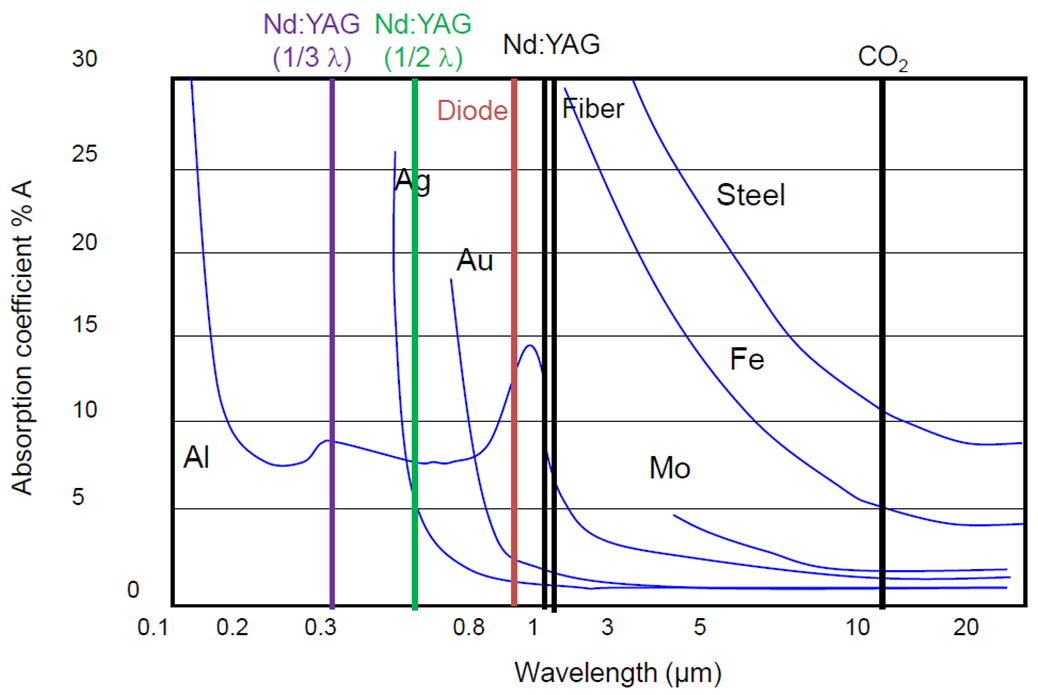
\includegraphics[width=0.75\linewidth]{imgs/abs.png}
	\caption{Coeficientes de absorción para diferentes familias de materiales.}
	\label{absfig}
\end{figure}

\begin{figure}[h!]
	\centering
	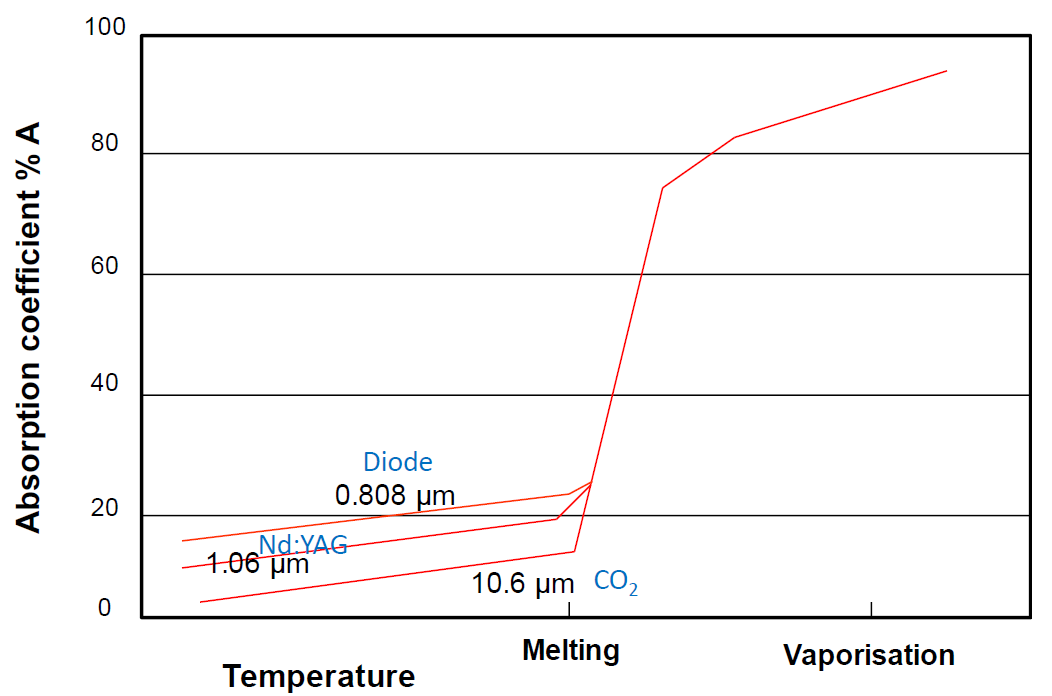
\includegraphics[width=0.65\linewidth]{imgs/hota.png}
	\caption{Cambio en el coeficiente de absorción con el aumento de temperatura en un metal.}
	\label{hotafig}
\end{figure}

El calor generado por la absorción en los elementos ópticos puede inducir deformaciones geométricas y cambios en la trayectoria del haz, afectando la precisión del sistema, por lo que nuevamente reconocemos la importancia de la refrigeración. Este principio es análogo al de la óptica en grandes telescopios astronómicos, donde la estabilidad térmica de los lentes se controla estrictamente para evitar errores de medida inducidos por dilataciones térmicas.  

En el caso de los láseres de \(\mathrm{CO_2}\), la transmisión del haz se realiza mediante espejos, siguiendo la ley de reflexión: el ángulo de incidencia es simétrico al ángulo de reflexión respecto a la normal del espejo. Así, la trayectoria del láser se controla modificando la orientación o posición de los espejos.  

\begin{equation}
	|\theta_{i}|=|\theta_{r}|
\end{equation}

Nótese que el valor es el mismo pero el signo debiese estrictamente ser opuesto, por el sentido en el cual se mide respecto en la vertical.

Estos espejos, típicamente de cobre para el caso de \(\mathrm{CO_2}\) (por su alta reflexión a esta longitud de onda), se desplazan junto con las estructuras montadas en los ejes CNC del cabezal de la máquina. Dado que una pequeña parte de la energía se absorbe en los espejos, estos suelen incorporar mecanismos de refrigeración, como canales de agua, para mantener la estabilidad térmica y preservar la precisión del haz. 

\subsection{Lentes}

Los lentes en los sistemas láser son componentes ópticos diseñados para modificar la dirección del haz de luz mediante el fenómeno de la refracción, determinado por la diferencia de índices de refracción entre medios y la geometría del lente. 

Como se mencionó anteriormente, un láser genera un haz coherente con divergencia muy reducida. Sin embargo, al salir de la fuente o al emerger de una fibra óptica, el haz puede presentar cierta divergencia. Esta divergencia se corrige mediante un \textbf{lente colimador}, cuya función es transformar el haz en un conjunto de rayos prácticamente paralelos.

El colimador se caracteriza principalmente por dos parámetros: su diámetro $d_{c}$ y su distancia focal $f_{col}$. Para lograr una colimación óptima, el lente debe colocarse a una distancia $f_{col}$ respecto al origen del haz, de modo que los rayos emergentes sean paralelos y mantengan la uniformidad del perfil (Figura \ref{lensesfig}).

\begin{figure}[h!]
	\centering
	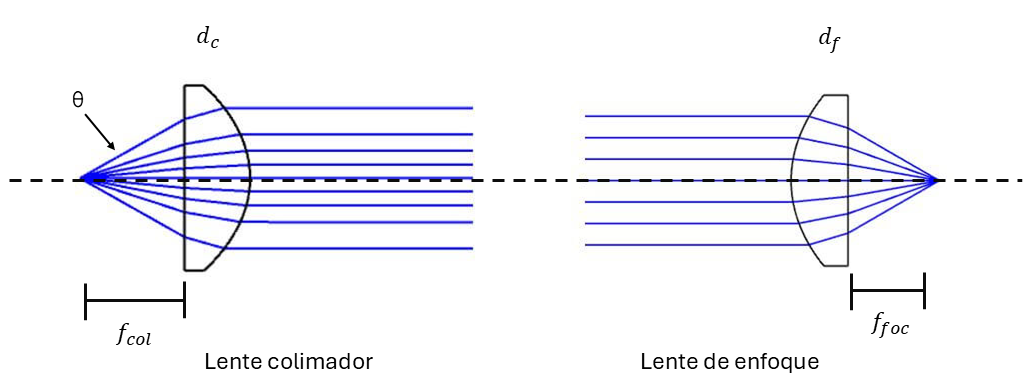
\includegraphics[width=0.8\linewidth]{imgs/lenses.png}
	\caption{Lente colimador y lente de enfoque.}
	\label{lensesfig}
\end{figure}

El haz colimado se dirige posteriormente hacia el \textbf{lente de enfoque}, que determina finalmente el diámetro del spot láser sobre el material objetivo. Este lente, con diámetro $d_{f}$, hace converger los rayos paralelos hacia un punto focal a una distancia denominada \textbf{distancia focal} $f_{foc}$, concentrando así la máxima intensidad del haz en la región de trabajo y asegurando la precisión del corte o procesamiento.


Un requisito fundamental en el diseño de lentes para sistemas láser es su tamaño. El diámetro efectivo del lente debe ser al menos igual o mayor que el diámetro del haz que se desea manipular; de lo contrario, parte de la energía del haz se perderá por recorte (\textit{clipping}), afectando tanto la eficiencia como la uniformidad del perfil de intensidad. En este sentido, el tamaño del haz a la salida de la fuente láser constituye un factor determinante para la selección del calibre de la óptica, ya que condiciona no solo la transmisión completa de la energía, sino también la calidad del enfoque y la minimización de aberraciones ópticas.

Es posible establecer una relación geométrica para evitar clipping, a través del ángulo de divergencia $\theta$, el diámetro de la fuente $d_{source}$ la distancia focal del colimador $f_{col}$ y el diámetro del lente colimador $d_{c}$ como:

\begin{equation}
	d_{c} \ge d_{\text{source}} + 2 f_{\text{col}} \tan(\theta)
\end{equation}

Para ángulos pequeños, como suele ser el caso en lásers, se puede aproximar la tangente directamente por el ángulo en radianes, además, el diámetro de la fuente suele ser bastante pequeño comparado con el diámetro del lente, luego:

\begin{equation}
	d_{c} \ge  2 f_{\text{col}}\theta
\end{equation}

\subsection{Fibra óptica}

La fibra óptica es un componente transparente y flexible que permite la transmisión de un haz de luz a lo largo de trayectorias arbitrarias, actuando como una guía óptica. Su principio de funcionamiento se basa en la \textbf{reflexión total interna}, que confina la luz dentro de la fibra.

Para comprender la transmisión en la fibra óptica, introducimos la \textbf{Ley de Snell} (Figura \ref{snelsfig}):

\begin{equation}
	n_i \sin\theta_i = n_t \sin\theta_t 
\end{equation}

donde los subíndices $i$ y $t$ corresponden al rayo incidente y transmitido, respectivamente. El coeficiente $n$ es el índice de refracción del medio, definido como:

\begin{equation}
	n = \frac{c}{v} 
\end{equation}

siendo $c$ la velocidad de la luz en el vacío y $v$ la velocidad de la luz en el medio. En general, el medio de entrada es aire, con $n_0 \approx 1$, de modo que al pasar a la fibra de índice $n_1$ se cumple:

\begin{equation}
	\sin\theta_1 = \frac{\sin\theta_0}{n_1} 
\end{equation}

\begin{figure}[h!]
	\centering
	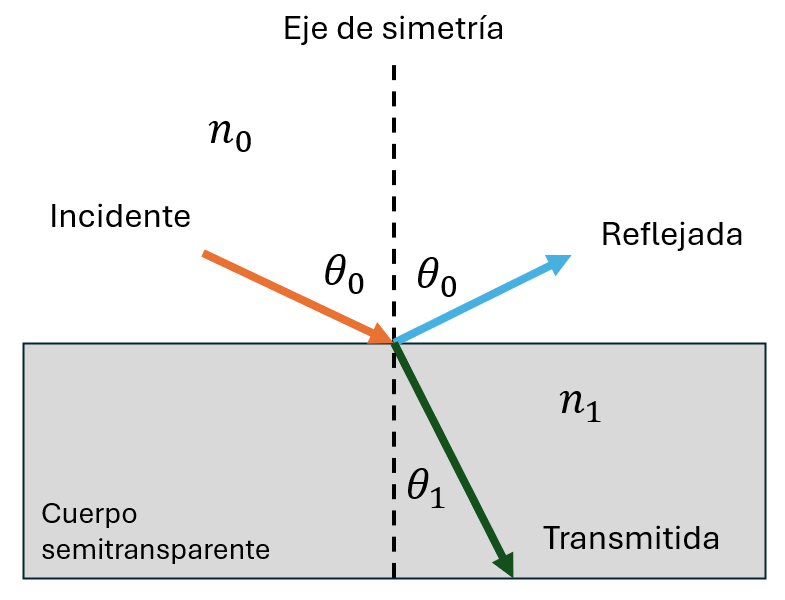
\includegraphics[width=0.55\linewidth]{imgs/snels.png}
	\caption{Ley de Snell.}
	\label{snelsfig}
\end{figure}

Una vez que el rayo ha ingresado a la fibra, este puede refractarse hacia el medio externo al llegar a la pared interna. Para impedir que escape, se requiere que la luz incidente sobre esa interfaz se refracte paralelo a la fibra. Así, el \textbf{ángulo crítico} $\theta_c$ del rayo moviéndose hacia la pared se obtiene imponiendo que el ángulo transmitido sea $\pi/2$ (Figura \ref{tirfig}):

\begin{equation}
	n_1 \sin\theta_c = n_2 \sin{\frac{\pi}{2}}
\end{equation}

De donde se obtiene:

\begin{equation}
	\sin\theta_c = \frac{n_2}{n_1} 
\end{equation}

Para asegurar esta condición, la fibra se recubre con un material concéntrico de índice ligeramente menor, denominado \textit{cladding} o \textbf{revestimiento}. Sobre el revestimiento se coloca una tercera capa de protección mecánica denominada \textit{buffer}. La parte de la fibra responsable del guiado óptico es entonces el \textbf{núcleo}.

\begin{figure}[h!]
	\centering
	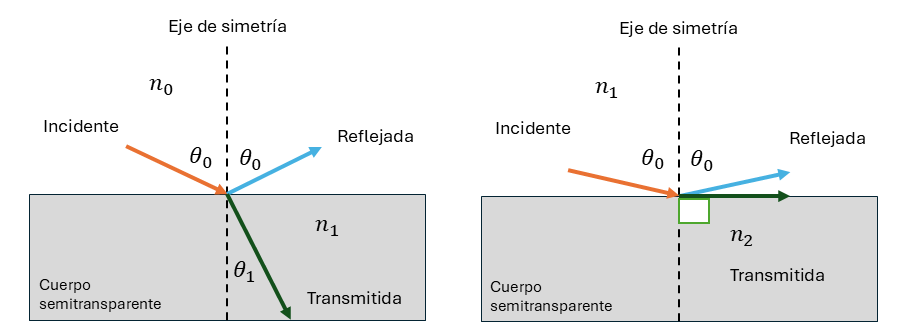
\includegraphics[width=0.9\linewidth]{imgs/tir.png}
	\caption{Caso general y caso de ángulo crítico para reflexión total interna.}
	\label{tirfig}
\end{figure}

A partir de la geometría de acoplamiento, se observa que la luz externa puede ingresar a la fibra solo si su ángulo de incidencia $\theta_0$ se encuentra dentro de un rango permitido, pues tiene relación con el $\theta_{c}$ que a su vez depende de los materiales de la fibra. Esto define el \textbf{cono de aceptación}, caracterizado por un semiángulo máximo $\theta_{\text{max}}$ (Figura \ref{fibropfig}).

\begin{figure}[h!]
	\centering
	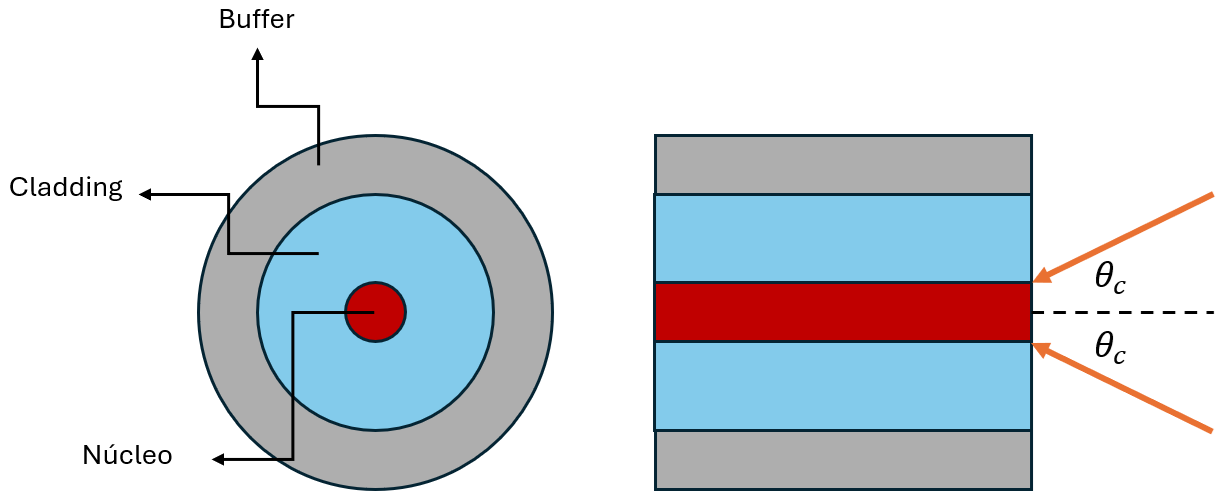
\includegraphics[width=0.8\linewidth]{imgs/fibrop.png}
	\caption{Estructura de la fibra óptica y cono de aceptación. }
	\label{fibropfig}
\end{figure}


Una forma conveniente de calcular este límite es mediante la \textbf{apertura numérica} (NA), definida como:

\begin{equation}
	\text{NA} = \sqrt{n_{1}^2 - n_{2}^2} 
\end{equation}

de modo que:

\begin{equation}
	\theta_{\text{max}} = \arcsin(\text{NA}) 
\end{equation}

De manera simétrica, esto definirá entonces el ángulo máximo para los rayos en la salida de la fibra.

Como la luz puede propagarse en distintos ángulos dentro del núcleo, los rayos recorren trayectorias ópticas distintas y pueden emerger con desfase. Este fenómeno se denomina \textbf{dispersión intermodal} y está asociado a la existencia de múltiples \textbf{modos de propagación} $M$, cuyo número depende del tamaño del núcleo y de la longitud de onda. Para mitigar este efecto, las fibras pueden presentar un índice escalonado o gradiente, como se ilustra en la Figura \ref{fig:modosm}. Esto se obtiene a través de un control de dopaje en la fabricación del núcleo.

\begin{figure}[h!]
	\centering
	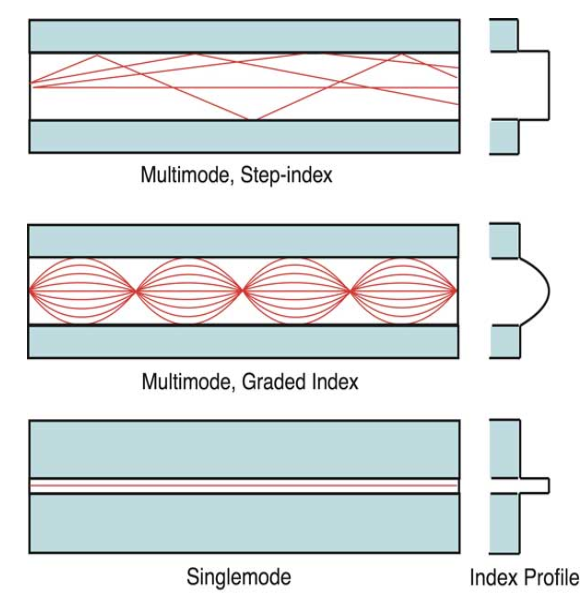
\includegraphics[width=0.5\linewidth]{imgs/mods.png}
	\caption{Perfiles de índice de refracción. \href{https://www.thefoa.org/tech/ref/basic/fiber.html}{Fuente}}
	\label{fig:modosm}
\end{figure}


Cabe notar que a pesar del diseño óptico de la fibra, no toda la energía se transporta, pues una pequeña parte de esta se absorbe, luego cada fibra presentará una pérdida relacionada a su longitud, con unidades típicamente de $dB/km$.

\section{Características de un láser}

Algunos atributos del láser dependen de forma inherente de las características de la fuente de emisión. Por su parte, la óptica de transmisión juega un papel determinante en las propiedades finales del spot láser, como su tamaño, forma y divergencia.

Un láser transporta la potencia suministrada por la fuente $P_{out}$ hasta la superficie del material de trabajo, donde se distribuye en el área del spot, el cual asumiremos circular de diámetro $d$. Este parámetro se conoce como \textbf{irradiancia} $I$, usualmente expresada en \si{\watt\per\centi\meter\squared}. De esta manera:

\begin{equation}
	I \propto \frac{P_{out}}{d}
\end{equation}

Como veremos a continuación, $I$ está lejos de ser una constante, pues presenta fluctuaciones tanto espaciales como temporales.

\subsection{Distribución espacial}

La sección transversal del spot láser generalmente no presenta una distribución de energía uniforme. 
Esta distribución está determinada por los modos transversales del campo electromagnético del resonador, denominados $TEM_{mn}$ (\textit{Transverse Electromagnetic Modes}), 
donde $m$ y $n$ definen la geometría del modo (ver Figura \ref{tems}).

\begin{figure}[h!]
	\centering
	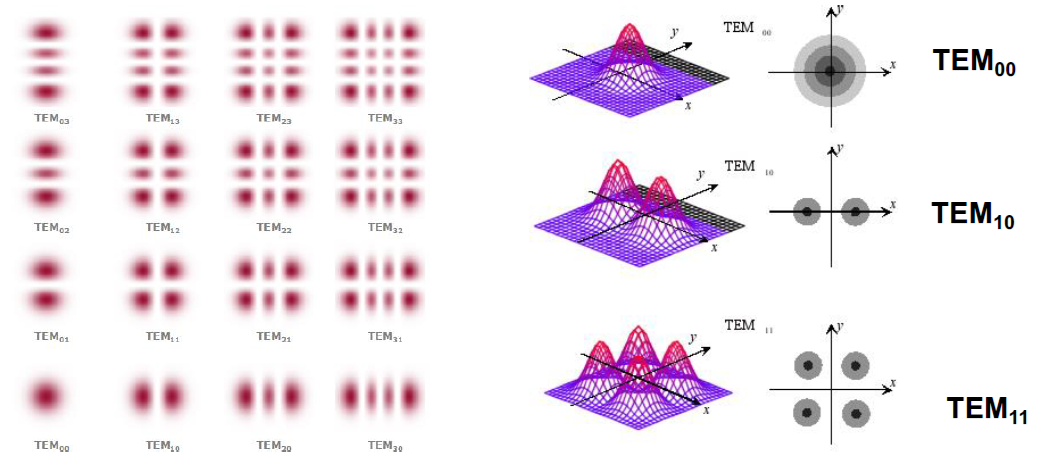
\includegraphics[width=1.0\linewidth]{imgs/tem.png}
	\caption{Modos transversales del campo electromagnético.}
	\label{tems}
\end{figure}

En la mayoría de los láseres empleados para fibras o procesos de propagación controlada, domina el modo fundamental $TEM_{00}$.
Este modo presenta una distribución gaussiana, muy concentrada en el centro e ideal para el enfoque.

Bajo la aproximación gaussiana estándar, la distribución de irradiancia en función del radio $r$ se escribe como:

\begin{equation}
	I(r) = I_0 \exp\!\left(-2\frac{r^2}{w_{0g}^2}\right),
\end{equation}

donde $I_0$ es la intensidad máxima y $w_{0g}$ es el \textbf{radio del haz} (\textit{beam waist radius}), definido como el valor de $r$ para el cual la intensidad cae a $I_0 / e^2$. Se usa la letra $w$ como referencia a \textit{waist} (cintura), pues como veremos más adelante, el perfil del láser toma una forma de hiperboloide con diámetro menor en la cintura.
Este parámetro es el utilizado en la caracterización estandarizada de haces (ISO 11146), podría variar de acuerdo a la referencia.

El diámetro correspondiente del haz es entonces:

\begin{equation}
	d_{0g} = 2w_{0g},
\end{equation}

Evaluando la distribución en $r = w_{0g}$:

\begin{equation}
	I(w) = I_0 e^{-2} \approx 0.135\, I_0,
\end{equation}

por lo que dentro del diámetro $d_{0g}$ se concentra aproximadamente el 86.5\% de la energía del haz gaussiano ideal (Figura \ref{gaussfig}).

\begin{figure}[h!]
	\centering
	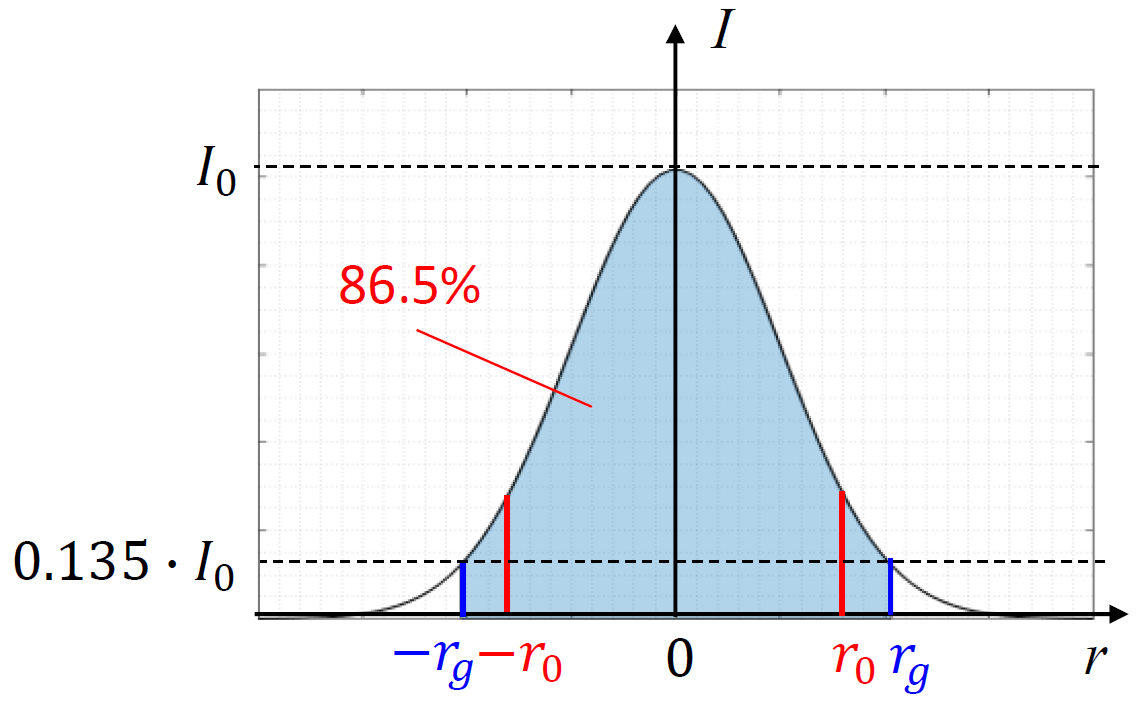
\includegraphics[width=0.75\linewidth]{imgs/gauss.png}
	\caption{Perfil gaussiano de irradiancia.}
	\label{gaussfig}
\end{figure}

Para un láser real, que puede contener modos superiores o desviarse del comportamiento gaussiano ideal, se introduce el \textbf{factor de calidad} del haz $M^2$. 
Este factor corrige el diámetro ideal para reflejar la propagación real del haz:

\begin{equation}
	d_{0} = M\, d_{0g}
\end{equation}

De esta manera, cuando se hable de un láser gaussiano se asumirá que $M^{2}=1$. Otra forma de definir este parámetro es como una razón entre el ángulo de divergencia del láser real $\theta$ respecto al ideal $\theta_{g}$ como:

\begin{equation}
	M^{2}=\frac{\theta}{\theta_{g}}
\end{equation}

El ángulo de divergencia de un láser real se puede calcular entonces como:

\begin{equation}
	\theta=M^{2}\frac{\lambda}{\pi w_{0g}}
\end{equation}

Otra forma de caracterizar la calidad de un láser es a través del \textit{beam parameter product}:

\begin{equation}
	BPP=\theta w_{0g}=M^{2}\frac{\lambda}{\pi}
\end{equation}

Esta divergencia debe ser tratada para la manipulación posterior del láser, para esto, usamos un lente colimador, el cual debe cumplir con la relación para evitar clipping (asumiendo la distribución gaussiana):

\begin{equation}
	d_{c}\approx 2f_{col}\theta = \frac{2 f_{col}\lambda M^{2}}{\pi d_{f}}
\end{equation}

Donde se usó una aproximación de ángulo pequeño y con $d_{f}$ el diámetro de la fibra. No es común colimar un láser proveniente de una fuente de CO2, pues presentan una divergencia relativamente despreciable.

Para aumentar la efectividad y precisión del láser, usamos un lente de enfoque a la salida para la convergencia de la energía en una zona más pequeña. La trayectoria de los rayos que convergen y luego divergen genera un hiperboloide, cuya sección más pequeña será entonces la cintura del láser. De esta forma, al variar el área del láser dependiendo de la profundidad, también lo hace la irradiancia.

El diámetro en la cintura del hiperboloide se puede calcular como:

\begin{equation}
	d_{0}=M^{2}\frac{4 \lambda f_{foc}}{\pi d_{c}}
\end{equation}

Para el caso de la transmisión por fibra se tiene la siguiente expresión:

\begin{equation}
	d_{0}=d_{f}\frac{f_{foc}}{f_{col}}=MA d_{f}
\end{equation}

Donde $MA$ es el factor de magnificación y $d_{f}$ el diámetro de la fibra.

El diámetro del spot láser será mínimo en la cintura, ubicada a $f_{foc}$ de distancia respecto al lente convergente, y presenta una variación simétrica en ambas direcciones. Desde este punto mediremos profundidad $z$, y será positivo en la dirección de propagación del láser. Si aproximamos el hiperboloide a un perfil triangular, para simplificar cálculos, llegamos a la siguiente expresión para estimar el diámetro del spot $d_{s}(z)$:

\begin{equation}
	d_{s}(z)=\sqrt{d_{0}^{2}+z^{2}(\frac{d_{c}}{f_{foc}})^{2}}
\end{equation}

Nótese que, mediante la aproximación de ángulos pequeños y siendo $d_{c}$ el diámetro del haz láser colimado:

\begin{equation}
	\frac{d_{c}}{f_{foc}}=\theta
\end{equation}

Luego, naturalmente, un mayor ángulo de convergencia (o menor $d_{c}$ o menor $f_{foc}$) genera una  mayor variación del diámetro al moverse en la profundidad $z$. Esta variación es importante, pues es deseable que el láser mantenga un nivel de irradiancia en cierto $\Delta z$ para poder trabajar con condiciones constantes en materiales de distinto espesor, por ejemplo. 

De esta manera, se define el \textbf{rango de Rayleigh} $z_{r}$ (Figura \ref{railifig}) a la distancia donde:

\begin{equation}
	r_{r}=\sqrt{2}w_{0}
\end{equation}

\begin{figure}[h!]
	\centering
	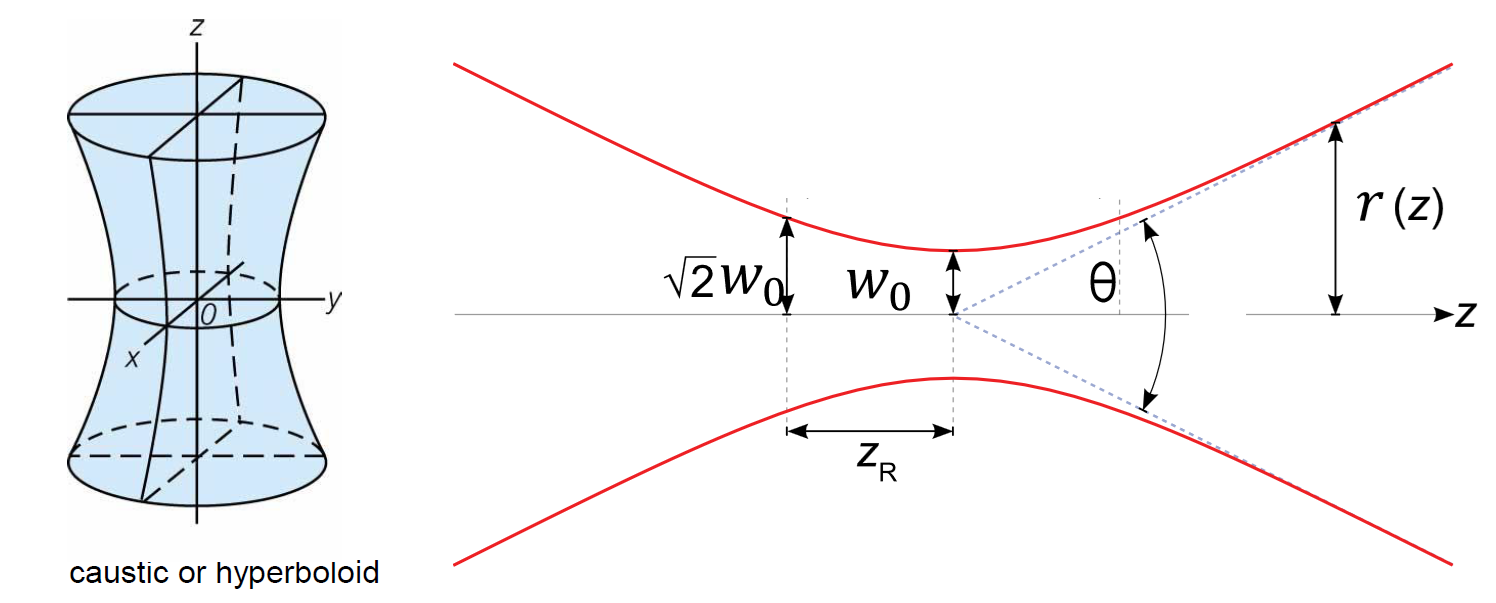
\includegraphics[width=0.75\linewidth]{imgs/raili.png}
	\caption{Perfil de hiperboloide para el láser en la salida y diagrama para la profundidad de campo.}
	\label{railifig}
\end{figure}

Lo cual corresponde al radio en el cual el área del spot se duplica. Desarrollando los cálculos, se tiene entonces que el rango de Rayleigh corresponde a:

\begin{equation}
	z_{r} = \frac{\pi d_{0}^{2}}{2 \lambda M^{2}}=2 \frac{d_{0} f_{foc}}{d_{c}}
\end{equation}

Por la simetría de la distribución, podemos entonces introducir la \textbf{profundidad de campo} (\textit{depth of field}), el cual indicará el espesor máximo de materiales que podemos tratar de manera efectiva:

\begin{equation}
DOF=2z_{r}
\end{equation}

\subsection{Distribución temporal}

El haz de luz se puede presentar en dos formas respecto a la naturaleza de la onda, pudiendo ser \textbf{continua} (\textit{CW, continuous wave}) o \textbf{pulsada} (\textit{PW, pulsed wave}) (Figura \ref{pulsedfig}).

\begin{figure}[h!]
	\centering
	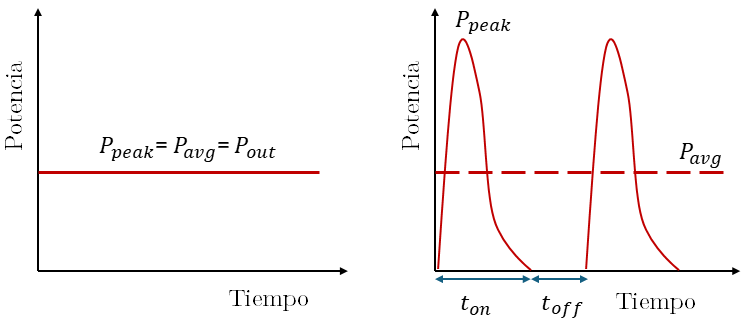
\includegraphics[width=0.85\linewidth]{imgs/pulsed.png}
	\caption{Perfil de onda continuo y pulsada.}
	\label{pulsedfig}
\end{figure}


La onda continua es naturalmente la más sencilla de tratar. Su potencia puede ser modulada previamente a la aplicación, y el perfil temporal es constante (con la potencia de salida igual a la promedio y al peak), luego:

\begin{equation}
	I = \frac{P_{out}}{A_{spot}}
\end{equation}

Las ondas pulsadas requieren más atención. Pulsar el láser significa que no está saliendo del resonador de manera constante como ocurre con la onda continua, sino que permanece un tiempo arbitrario aumentando su densidad energética antes de emerger. De esta manera, cada pulso emitido puede transportar una vasta cantidad de energía.  

Para estimar esta energía, primero consideramos la potencia nominal o promedio que entrega la fuente del sistema láser y calculamos la energía total en un pulso de frecuencia $f$ como:

\begin{equation}
	E = \frac{P_{out}}{f}
\end{equation}

El pulso puede tener distintas formas, pero para simplificación de los cálculos, asumiremos que la onda siempre es cuadrada. Podemos caracterizar una onda cuadrada a través de los tiempos de encendido $t_{on}$ y apagado $t_{off}$, definiendo el \textbf{factor de ocupación} o \textit{duty cycle}:

\begin{equation}
	\delta = \frac{t_{on}}{t_{tot}} = \frac{t_{on}}{t_{on}+t_{off}}
\end{equation}

De esta manera, si $t_{on}$ corresponde al tiempo de encendido de la onda, la \textbf{potencia peak} en ese lapso es:

\begin{equation}
	P_{peak} = \frac{E}{t_{on}} = P_{out}\delta 
\end{equation}

Las potencias peak que alcanza un láser pulsado van desde los W hasta los MW, por lo que se separa la duración de los pulsos en categorías, pues generan distintas interacciones con la materia.

Dado que el tiempo de acción del láser sobre un material define la transferencia de calor, definimos la \textbf{fluencia} como una medida para caracterizar un láser pulsado (típicamente en $\si{\J\per\centi\meter\squared}$):

\begin{equation}
	F = \frac{E}{A}
\end{equation}

Es la fluencia el parámetro clave que usaremos para definir qué mecanismo de corte actuará sobre un material para un setup dado.

Para encontrar un equivalente en un sistema láser continuo, es necesario considerar un tiempo de interacción de manera análoga:

\begin{equation}
	F_{CW} = I \cdot t_{inter} \approx I \cdot \frac{d}{v}
\end{equation}

Donde aproximamos este tiempo a través del tamaño del spot $d$ y la velocidad de avance lineal $v$ del cabezal.

\section{Interacción láser}

\subsection{Mecanismos de acción}

Una vez que el haz láser emerge de la óptica e interactúa con el material, no toda la potencia o energía resulta efectiva en el proceso. Esto depende del coeficiente de absorción del material para la longitud de onda del láser. Dicho coeficiente puede incorporarse al inicio del análisis —ajustando la potencia nominal disponible— o bien directamente en la expresión de irradiancia, por ejemplo:

\begin{equation}
	I = \frac{A \, P_{out}}{A_{spot}}
\end{equation}

donde $A$ es el coeficiente de absorción del material. Se utiliza el subíndice spot para evitar confusiones entre el área y la absorción.

Al tratarse de un proceso térmico, la energía depositada por el láser se distribuye en el material de acuerdo con sus propiedades termofísicas. El aumento de temperatura puede producir distintas consecuencias: simple calentamiento, alteración de la microestructura, fusión o vaporización.

Un mayor tiempo de interacción implica naturalmente una mayor energía entregada, pero también permite una mayor difusión térmica hacia regiones no deseadas. Esto incrementa la zona afectada térmicamente (\textit{heat-affected zone}, HAZ), lo cual suele ser indeseable.

Por ello, utilizamos la \textbf{fluencia} del sistema para compararla con los umbrales característicos del material y determinar cuál será el mecanismo de interacción predominante (Figura \ref{mechsfig}), como se ilustra en el Cuadro \ref{fluencias}.

\begin{table}[h!]
	\centering
	\caption{Rangos típicos de fluencia en $\si{\J\per\centi\meter\squared}$ para mecanismos de acción predominante en acero al carbono (A36–1020).}
	\label{fluencias}
	\begin{tabular}{|c|c|c|c|c|}
		\hline
		\textbf{Calentamiento} &
		\textbf{Cambio de microestructura} &
		\textbf{Fusión} &
		\textbf{Vaporización} &
		\textbf{Ablación} \\
		\hline
		0.05--0.5 &
		0.5--5 &
		5--20 &
		20--60 &
		60--150 \\
		\hline
	\end{tabular}
\end{table}

\begin{figure}[h!]
	\centering
	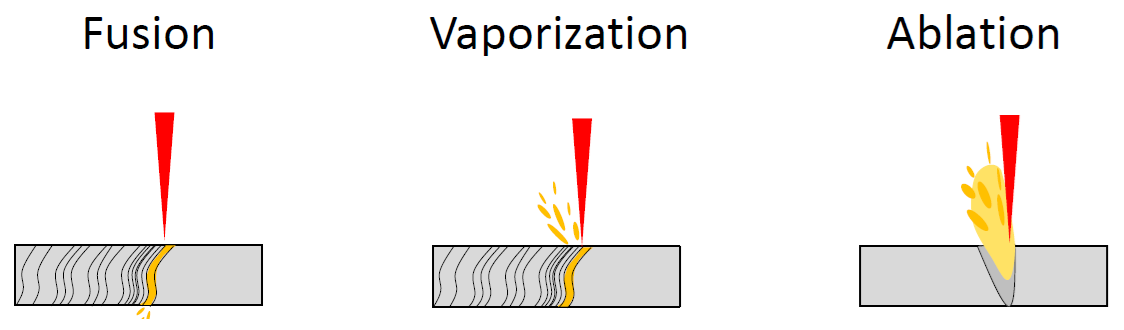
\includegraphics[width=0.9\linewidth]{imgs/mechs.png}
	\caption{Mecanismos térmicos donde se genera remoción.Nótese que en fusión el material fluye hacia abajo, mientras que en vaporizacion y ablación difunde hacia arriba.}
	\label{mechsfig}
\end{figure}

El tipo de mecanismo para definir el setup depende del proceso que se desee realizar. Por ejemplo, en soldadura se busca fundir el material sin removerlo, mientras que un corte limpio se obtiene en el régimen de vaporización, y aún más, mediante \textbf{ablación}.

La ablación es un mecanismo en el cual la energía incidente sobre el material es lo suficientemente intensa como para romper los enlaces interatómicos sin que se produzca una difusión significativa del calor. Esto permite un maquinado muy preciso, de alta calidad y con una zona afectada por el calor (HAZ) mínima. Este tipo de mecanismo es característico de los sistemas láser pulsados.

\subsection{Modelos térmicos}

Hasta ahora, hemos mencionado parámetros de interacción y propios de la máquina para caracterizar al láser, los cuales corresponden a la herramienta de este proceso. A diferencia de otras tecnologías abordadas en este texto, no es directo definir el ancho y la profundidad de corte que se obtienen con el láser.

Como se sabe, el láser entrega energía al material, elevando su temperatura y, eventualmente, generando algún cambio deseado, ya sea fusión, vaporización o ablación. Por lo tanto, se requiere un modelo térmico que permita estimar el campo de temperaturas para cuantificar y precisar los efectos de los parámetros configurados.

Los modelos de transferencia de calor para este tipo de procesos suelen ser multivariables, iterativos y con altos tiempos de cómputo. No obstante, existen modelos simplificados que permiten aproximar de manera efectiva ciertos tipos de interacción.

Uno de los más utilizados es el \textbf{modelo conductivo}, basado en la Ley de Fourier y una serie de supuestos sobre el comportamiento del material y la distribución de energía del láser. En este modelo, la distribución espacial del láser se representa mediante la función $\mathrm{ierfc}$, la integral del error complementario:

\begin{equation}
	T(x,y,z,t) = T_0 + \frac{I}{k \sqrt{\pi \alpha t}} \, 
	\mathrm{ierfc}\left(\frac{\sqrt{x^2 + y^2 + (c_z z)^2}}{2\sqrt{\alpha t}}\right),
\end{equation}

donde $T(x,y,z,t)$ es la temperatura en la posición $(x,y,z)$ y tiempo $t$, $T_0$ la temperatura inicial del material, $I$ la irradiancia del láser, $k$ la conductividad térmica, $\alpha$ la difusividad térmica y $c_z$ un factor de corrección en la dirección $z$. Esta formulación permite obtener un perfil tridimensional aproximado de temperatura bajo ciertas condiciones de conducción térmica dominante.

A través de este modelo, podemos hacer comparaciones teóricas, como la que se observa en la Figura \ref{stilgoldfig}. Aquí se puede notar que el acero alcanza mayores temperaturas cerca de la superficie, mientras que el oro difunde la energía con mayor efectividad, aumentando la profundidad afectada pero disminuyendo el valor máximo.

Una adaptación de este enfoque es el \textbf{modelo de Rosenthal}, que estima la geometría del área afectada por un láser mediante un modelo de conducción semi-estacionario:

\begin{equation}
	\begin{aligned}
		T(x, y, z) =& T_0 + \frac{P}{2 \pi k R} \exp\left(-\frac{v (x + R)}{2 \alpha}\right), \\[0.5em]
		R =& \sqrt{x^2 + y^2 + (c_z z)^2},
	\end{aligned}
\end{equation}

donde $T_0$ es la temperatura inicial, $P$ la potencia del láser, $k$ la conductividad térmica del material, $v$ la velocidad de desplazamiento del láser en dirección $x$ y $\alpha$ la difusividad térmica del material. La variable $R$ representa la distancia efectiva desde el punto de aplicación de energía y $c_z$ ajusta la propagación en profundidad. Este modelo no requiere iteración: propaga la ecuación de calor directamente en el dominio espacial y temporal.

\begin{figure}[h!]
	\centering
	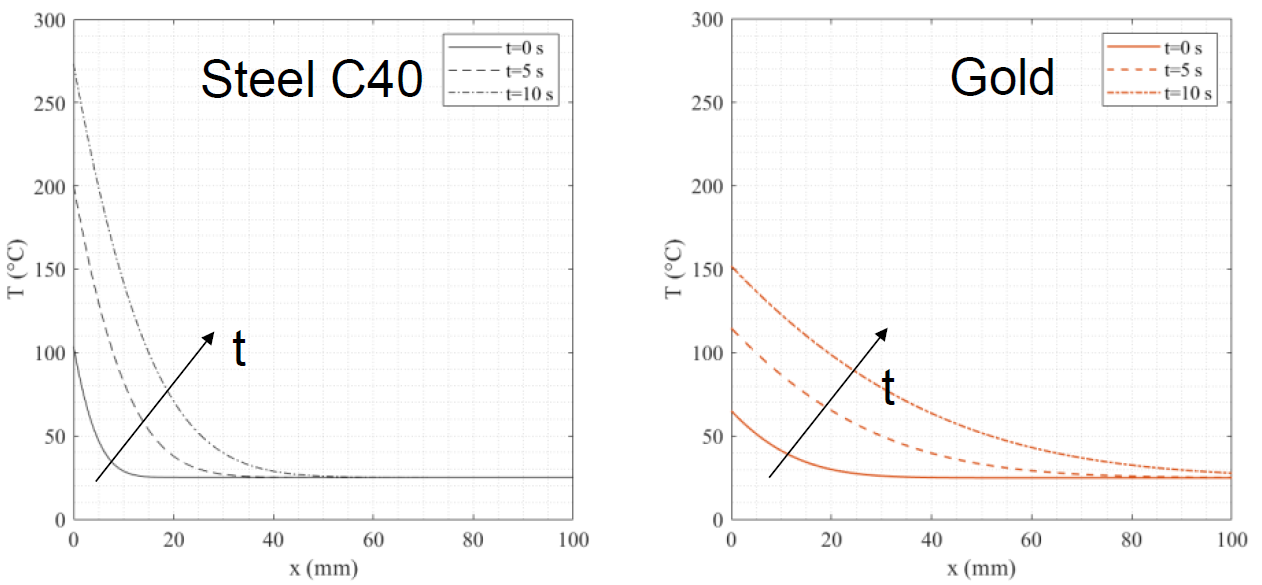
\includegraphics[width=1.0\linewidth]{imgs/stilgold.png}
	\caption{Valores de temperatura en función de la profundidad para dos materiales.}
	\label{stilgoldfig}
\end{figure}

El resultado son campos de temperatura, como se observa en la Figura \ref{contorfig}. A través de las curvas de nivel, es posible estimar el ancho del corte, así como la profundidad, tras calibrar el modelo con datos experimentales.

Estos modelos simplificados proporcionan una aproximación o metodología para abordar nuevas condiciones de trabajo. No obstante, en la práctica, las empresas suelen generar sus propios datos basándose en experiencia y establecen configuraciones estándar para cada proceso.

Actualmente, las nuevas máquinas láser incluyen \textbf{settings precalibrados} para una biblioteca de materiales y espesores, sobre los cuales el usuario puede realizar ajustes adicionales. Esto refleja que predecir de manera exacta la acción del corte con láser sigue siendo una tarea compleja y dependiente de múltiples variables.

\begin{figure}[h!]
	\centering
	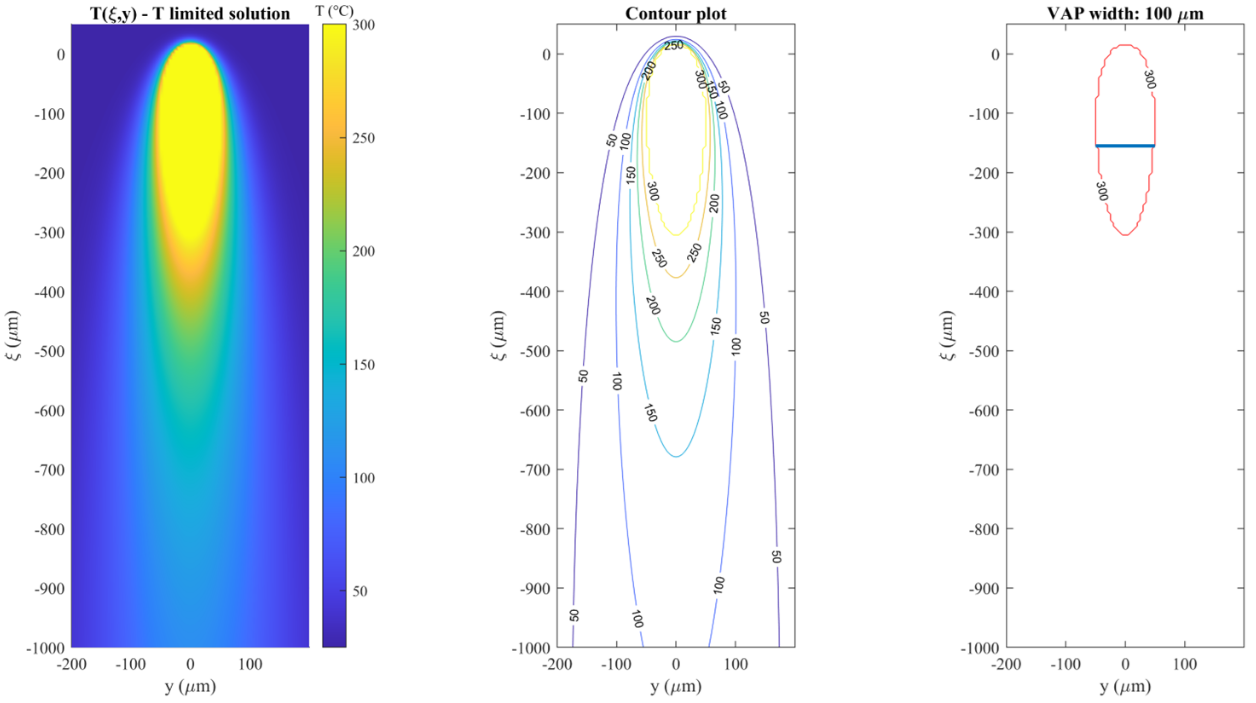
\includegraphics[width=1.0\linewidth]{imgs/contor.png}
	\caption{Campo de temperaturas simulado mediante el modelo de Rosenthal.}
	\label{contorfig}
\end{figure}

\subsection{Procesos de corte láser}

En la industria, los procesos de remoción láser más comunes utilizan las siguientes operaciones básicas:

\begin{itemize}
	\item \textbf{Contorneado:} El láser sigue $n$ pasadas sobre el contorno de una geometría para separarla del material base. Esta operación puede incluir \emph{tabs}, al igual que ocurre en el contorneado con fresado.
	\item \textbf{Grabado de contorno:} Similar al contorneado, pero con menor profundidad, destinado a generar una diferencia visual o marca superficial sin atravesar completamente el material.
	\item \textbf{Grabado de área:} En este caso, también de baja profundidad, se define un patrón de rasterizado que cubre toda el área objetivo. Este patrón puede ser preconfigurado o vectorizado de manera personalizada, controlando el \emph{overlap} entre pasadas y la dirección de barrido.
\end{itemize}

Por lo general, las máquinas láser de escritorio presentan limitaciones en la configuración de parámetros. Típicamente, es posible modular la potencia $P$, la velocidad de avance $v$ y el número de pasadas $n$. El material se suele enfocar previamente a la ejecución del corte, y únicamente los modelos de mayor costo permiten un ajuste automático de la distancia focal durante la operación.

Un modelo sencillo para estimar los parámetros de corte se basa en la \textbf{capacidad térmica} del material y el dimensionamiento del volumen a remover (Figura \ref{kreffig}):

\begin{equation}
	P = w \, h \, v \, \rho \left[ c_{p}(T_{m}-T_{0}) + L_{m} + m' L_{v} \right]
\end{equation}

donde:  
\begin{itemize}
	\item $w$ es el ancho de corte, que puede aproximarse mediante el diámetro del haz $d_s$.
	\item $h$ es la profundidad de corte.
	\item $\rho$ es la densidad del material.
	\item $c_p$ es la capacidad calorífica.
	\item $T_m$ y $T_0$ son la temperatura de fusión y la temperatura inicial, respectivamente.
	\item $L_m$ y $L_v$ son las entalpías de fusión y vaporización.
	\item $m'$ representa la fracción de material que se evapora.
\end{itemize}

\begin{figure}[h!]
	\centering
	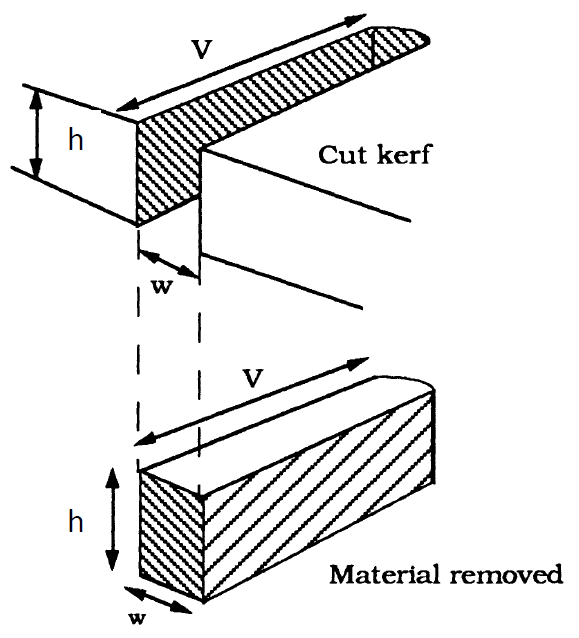
\includegraphics[width=0.5\linewidth]{imgs/kref.png}
	\caption{Material removido mediante el corte.}
	\label{kreffig}
\end{figure}

De esta manera, dado un \emph{setup} fijo, es posible estimar velocidades admisibles de referencia para la operación deseada.


\subsection{Sistemas de corte láser}

Respecto a los métodos de corte láser, los sistemas pueden clasificarse en dos tipos según la proximidad del cabezal con el material: \textbf{de proximidad} y \textbf{remotos} (Figura \ref{proxfig}). Esta distinción influye directamente en la calidad del corte, la velocidad de operación y la elección del gas de asistencia.

\begin{figure}[h!]
	\centering
	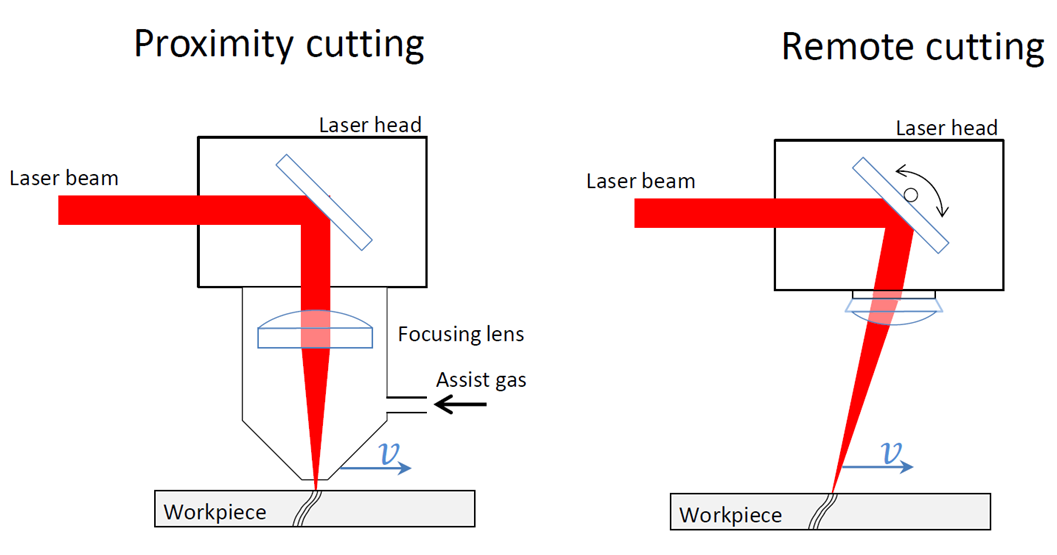
\includegraphics[width=0.8\linewidth]{imgs/prox.png}
	\caption{Material removido mediante el corte.}
	\label{proxfig}
\end{figure}

En los sistemas de \textbf{proximidad}, el cabezal mantiene una distancia \textbf{stand-off} de algunos milímetros respecto al material. Desde este cabezal se inyectan gases de asistencia, que pueden ser \textbf{inertes} o \textbf{reactivos}.  

Los gases \textbf{inertes} cumplen varias funciones: evacuar el material fundido y vaporizado, prevenir la oxidación en metales y proteger la óptica del sistema. Su uso permite obtener un acabado superficial más limpio y una zona afectada por calor (\textbf{HAZ}) mínima.  

Por otro lado, los gases \textbf{reactivos}, como el oxígeno, inducen oxidación en el material, generando una reacción exotérmica que incrementa la energía disponible para el corte. En este caso, el láser solo debe suministrar periódicamente la energía de activación necesaria para mantener la reacción. Como se observa en la Figura \ref{reactfig}, el uso de un gas reactivo puede aumentar la velocidad de corte, aunque la terminación superficial suele ser menos uniforme y el \textbf{HAZ} más amplio que en el caso de gases inertes.

\begin{figure}[h!]
	\centering
	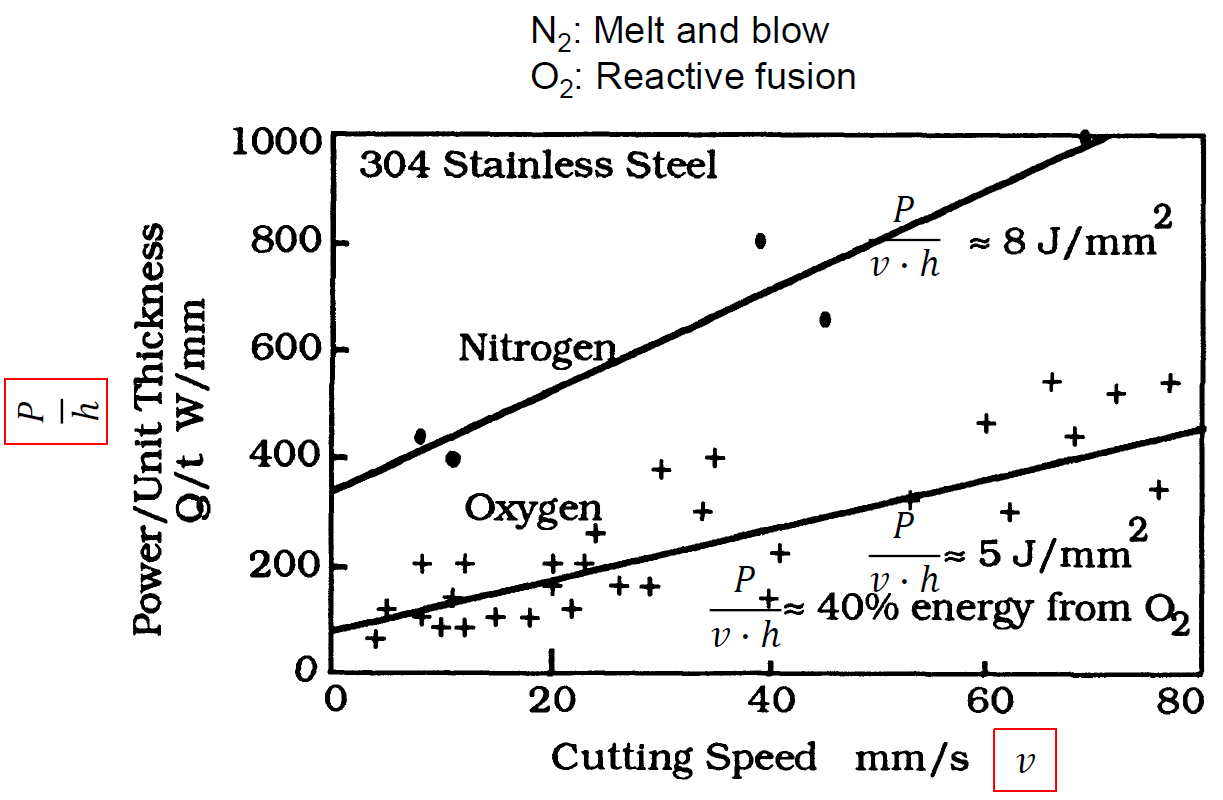
\includegraphics[width=0.7\linewidth]{imgs/blow.png}
	\caption{Comparación de parámetros de corte para un mismo material, por evacuación y por reacción.}
	\label{reactfig}
\end{figure}

La terminación de un corte por contorno generalmente presenta un estriado, así como una fracción de material fundido que puede escurrir hacia el borde inferior de la sección (Figura \ref{qualityfig}), facilitada por los gases de evacuación. Tanto el inicio como el final del corte suelen mostrar una acumulación triangular de material donde la penetración es incompleta respecto al resto del perímetro. Esto ocurre porque, en estas zonas, la velocidad del cabezal cambia y el campo de temperaturas es relativamente más bajo. Estas irregularidades se corrigen mediante estrategias específicas, como pasadas adicionales, variación de la potencia del láser o el uso de \emph{tabs} temporales.

En los sistemas \textbf{remotos}, el láser se propaga a través de espejos y el cabezal se mantiene a mayor distancia del material, sin necesidad de gases de asistencia, aunque pueden tener esa opción. Esta configuración reduce la inercia del cabezal, lo que permite alcanzar mayores velocidades de desplazamiento. También, ofrece mayor seguridad al mantener el cabezal alejado de la zona de corte.  

Los sistemas remotos requieren un enfoque óptico más preciso, ya sea mediante una distancia focal elevada o una divergencia pequeña del haz. 

\begin{figure}[h!]
	\centering
	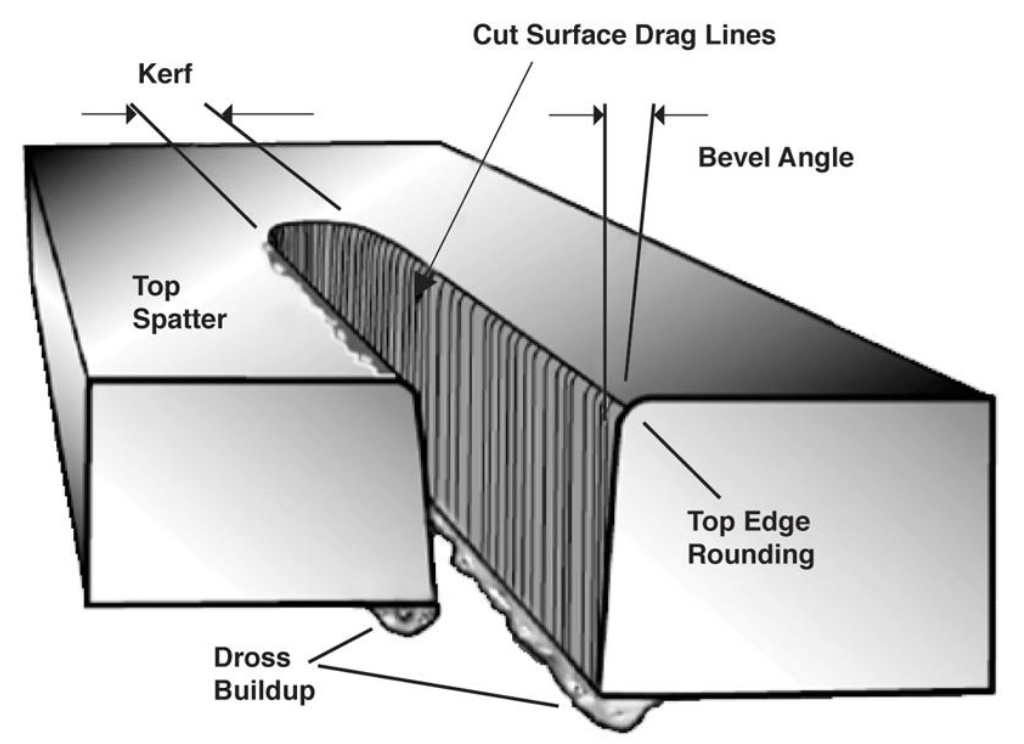
\includegraphics[width=0.6\linewidth]{imgs/quality.png}
	\caption{Calidad de un corte láser.}
	\label{qualityfig}
\end{figure}

